\documentclass[tikz,border=2pt]{standalone}
\usepackage{pgfplots}
\pgfplotsset{compat=1.18}
\usepgfplotslibrary{fillbetween}

% Colorblind-safe, print-friendly palette. Marker shapes and line styles retain
% the distinctions when the figure is printed in grayscale.
\definecolor{dfblack}{HTML}{202124}
\definecolor{familyblue}{HTML}{0072B2}
\definecolor{hoeffdingorange}{HTML}{D55E00}
\definecolor{alphaGreen}{HTML}{20854E}
\definecolor{alphaPurple}{HTML}{7655A3}
\definecolor{alphaRed}{HTML}{B53A3A}
\definecolor{auditgray}{HTML}{EEF1F4}
\definecolor{bordergray}{HTML}{69737D}

\begin{document}
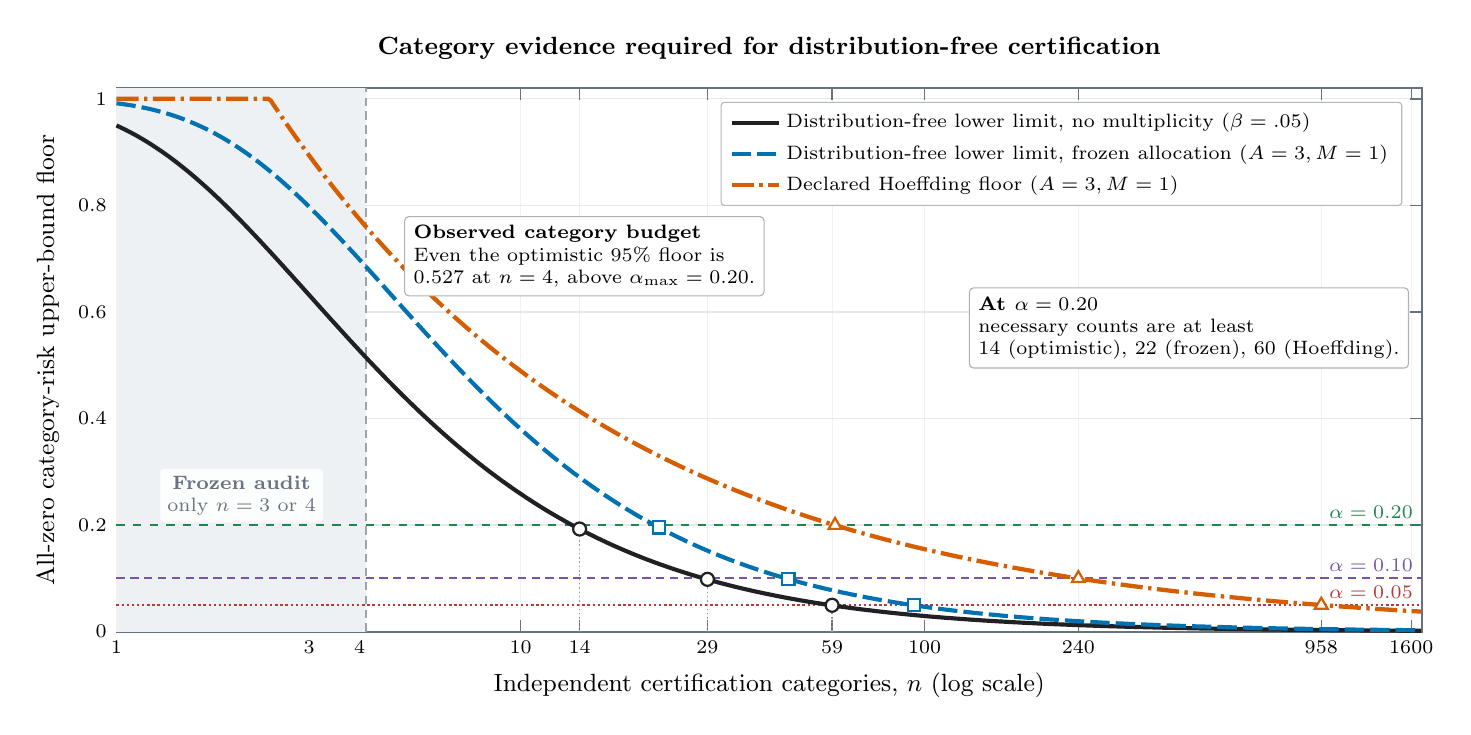
\begin{tikzpicture}
\begin{axis}[
    width=7.15in,
    height=3.34in,
    xmode=log,
    log basis x=10,
    xmin=1,
    xmax=1700,
    ymin=0,
    ymax=1.02,
    axis line style={line width=0.65pt,draw=bordergray},
    tick style={line width=0.55pt,draw=bordergray},
    xmajorgrids=true,
    ymajorgrids=true,
    x grid style={gray!11,line width=0.35pt},
    y grid style={gray!18,line width=0.45pt},
    xlabel={Independent certification categories, $n$ (log scale)},
    ylabel={All-zero category-risk upper-bound floor},
    title={Category evidence required for distribution-free certification},
    title style={font=\small\bfseries,yshift=1pt},
    label style={font=\small},
    tick label style={font=\scriptsize},
    legend style={
        at={(0.985,0.975)},
        anchor=north east,
        font=\scriptsize,
        draw=bordergray!50,
        rounded corners=1.2pt,
        fill=white,
        fill opacity=0.97,
        text opacity=1,
        cells={anchor=west},
        row sep=0.5pt
    },
    xtick={1,3,4,10,14,29,59,100,240,958,1600},
    xticklabels={1,3,4,10,14,29,59,100,240,958,1600},
    ytick={0,0.2,0.4,0.6,0.8,1.0},
    clip=false,
]

% The frozen archive supplies only three or four distinct certification
% categories. The label is placed in the empty lower part of the band so no
% analytic curve crosses the text.
\path[fill=auditgray,draw=none]
    (axis cs:1,0) rectangle (axis cs:4.15,1.02);
\draw[bordergray!65,densely dashed,line width=0.7pt]
    (axis cs:4.15,0) -- (axis cs:4.15,1.02);
\node[
    anchor=center,
    font=\scriptsize,
    text=bordergray,
    align=center,
    fill=white,
    fill opacity=0.88,
    text opacity=1,
    rounded corners=1pt,
    inner sep=2.5pt
] at (axis cs:2.04,0.255)
{\textbf{Frozen audit}\\only $n=3$ or $4$};

% Requested operating levels are drawn before the analytic curves, so the
% primary data strokes remain visually dominant at every crossing.
\addplot[forget plot,alphaGreen,dashed,line width=0.75pt] coordinates {(1,0.20) (1700,0.20)};
\addplot[forget plot,alphaPurple,dash pattern=on 3pt off 2pt,line width=0.70pt]
    coordinates {(1,0.10) (1700,0.10)};
\addplot[forget plot,alphaRed,densely dotted,line width=0.85pt]
    coordinates {(1,0.05) (1700,0.05)};

% Analytic all-zero floors. The M=1 curves are deliberately the most
% favorable frozen allocation; Table 1 reports M=5 and M=20 as well.
\addplot[dfblack,line width=1.50pt,domain=1:1700,samples=500]
    {1 - 0.05^(1/x)};
\addlegendentry{Distribution-free lower limit, no multiplicity ($\beta=.05$)}

\addplot[familyblue,dash pattern=on 7pt off 2.2pt,line width=1.50pt,domain=1:1700,samples=500]
    {1 - (0.05/6)^(1/x)};
\addlegendentry{Distribution-free lower limit, frozen allocation ($A=3,M=1$)}

\addplot[hoeffdingorange,dash pattern=on 8pt off 2pt on 1.2pt off 2pt,line width=1.55pt,domain=1:1700,samples=500]
    {min(1,sqrt(ln(120)/(2*x)))};
\addlegendentry{Declared Hoeffding floor ($A=3,M=1$)}

% Direct labels sit on opaque white pads and cannot be crossed by a curve.
\node[anchor=south east,font=\scriptsize,text=alphaGreen,fill=white,inner sep=1.2pt]
    at (axis cs:1650,0.205) {$\alpha=0.20$};
\node[anchor=south east,font=\scriptsize,text=alphaPurple,fill=white,inner sep=1.2pt]
    at (axis cs:1650,0.105) {$\alpha=0.10$};
\node[anchor=south east,font=\scriptsize,text=alphaRed,fill=white,inner sep=1.2pt]
    at (axis cs:1650,0.055) {$\alpha=0.05$};

% Optimistic distribution-free crossings: 14, 29, and 59 categories.
\addplot[forget plot,only marks,mark=*,mark size=2.35pt,fill=white,draw=dfblack,line width=0.8pt]
    coordinates {(14,0.1926362) (29,0.0981446) (59,0.0495076)};
\draw[dfblack!45,densely dotted,line width=0.55pt] (axis cs:14,0) -- (axis cs:14,0.1926362);
\draw[dfblack!45,densely dotted,line width=0.55pt] (axis cs:29,0) -- (axis cs:29,0.0981446);
\draw[dfblack!45,densely dotted,line width=0.55pt] (axis cs:59,0) -- (axis cs:59,0.0495076);
% Frozen-allocation DF crossings: 22, 46, and 94.
\addplot[forget plot,only marks,mark=square*,mark size=2.2pt,fill=white,draw=familyblue,line width=0.8pt]
    coordinates {(22,0.1955635) (46,0.0988431) (94,0.0496555)};

% Favorable M=1 Hoeffding crossings: 60, 240, and 958.
\addplot[forget plot,only marks,mark=triangle*,mark size=2.65pt,fill=white,draw=hoeffdingorange,line width=0.8pt]
    coordinates {(60,0.1997392) (240,0.0998696) (958,0.0499869)};

\node[
    anchor=north west,
    font=\scriptsize,
    align=left,
    fill=white,
    draw=bordergray!55,
    rounded corners=1.5pt,
    inner sep=3.2pt
] at (axis cs:5.15,0.78)
{\textbf{Observed category budget}\\Even the optimistic 95\% floor is\\$0.527$ at $n=4$, above $\alpha_{\max}=0.20$.};

\node[
    anchor=east,
    font=\scriptsize,
    align=left,
    fill=white,
    draw=bordergray!55,
    rounded corners=1.5pt,
    inner sep=3.2pt
] at (axis cs:1580,0.57)
{\textbf{At $\alpha=0.20$}\\necessary counts are at least\\14 (optimistic), 22 (frozen), 60 (Hoeffding).};

\end{axis}
\end{tikzpicture}
\end{document}
